\documentclass[t]{beamer}
\mode<presentation>

\usepackage{etex}

\usetheme{Madrid}
% other themes: Warsaw, AnnArbor, Antibes, Bergen, Berkeley, Berlin, Boadilla, boxes, CambridgeUS, Copenhagen, Darmstadt, default, Dresden, Frankfurt, Goettingen,
% Hannover, Ilmenau, JuanLesPins, Luebeck, Madrid, Maloe, Marburg, Montpellier, PaloAlto, Pittsburg, Rochester, Singapore, Szeged, classic

\setbeamertemplate{navigation symbols}{\insertslidenavigationsymbol}

\usecolortheme{dolphin}
%\usecolortheme{seagull}
% color themes: albatross, beaver, beetle, crane, default, dolphin, dov, fly, lily, orchid, rose, seagull, seahorse, sidebartab, structure, whale, wolverine

%\usefonttheme{serif}
% font themes: default, professionalfonts, serif, structurebold, structureitalicserif, structuresmallcapsserif

% pdf is displayed in full screen mode automatically
%\hypersetup{pdfpagemode=FullScreen}

%\AtBeginSection[]
%{
%  \begin{frame}<beamer>
%    \frametitle{Outline}
%    \tableofcontents[currentsection,currentsubsection]
%  \end{frame}
%}

% define your own colours:
\definecolor{Red}{rgb}{1,0,0}
\definecolor{Blue}{rgb}{0,0,1}
\definecolor{Green}{rgb}{0,1,0}
\definecolor{magenta}{rgb}{1,0,.6}
\definecolor{lightblue}{rgb}{0,.8,1}
\definecolor{lightpurple}{rgb}{.6,.4,1}
\definecolor{gold}{rgb}{.6,.5,0}
\definecolor{orange}{rgb}{1,0.4,0}
\definecolor{hotpink}{rgb}{1,0,0.5}
\definecolor{newcolor2}{rgb}{.5,.3,.5}
\definecolor{newcolor}{rgb}{0,.3,1}
\definecolor{newcolor3}{rgb}{1,0,.35}
\definecolor{darkgreen1}{rgb}{0, .35, 0}
\definecolor{darkgreen}{rgb}{0, .6, 0}
\definecolor{darkred}{rgb}{.75,0,0}

\xdefinecolor{olive}{cmyk}{0.64,0,0.95,0.4}
\xdefinecolor{purpleish}{cmyk}{0.75,0.75,0,0}

%\usepackage{beamerinnerthemerounded}
% inner themes include circles, default, inmargin, rectangles, rounded

%\usepackage{beamerouterthemesmoothbars}
% outer themes include default, infolines, miniframes, shadow, sidebar, smoothbars, smoothtree, split, tree

\useoutertheme[subsection=false]{smoothbars}

% to have the same footer on all slides
\setbeamertemplate{footline}[text line]{
\raisebox{3pt}{
\includegraphics[height=15pt]{su-long.eps}}\hfill 
\raisebox{5pt}{Math 207:  Statistics}\hfill 
\raisebox{5pt}{Law of Averages}\hfill
\raisebox{5pt}{\insertframenumber/\pageref{lastpage}}}
%\setbeamertemplate{footline}[text line]{} % or empty footer

% include packages
\usepackage{subfigure}
\usepackage{multicol}
\usepackage{amsmath}
\usepackage{epsfig}
\usepackage{graphicx}
\usepackage[all,knot]{xy}
\xyoption{arc}
\usepackage{url}
\usepackage{multimedia}
\usepackage{hyperref}
\usepackage{setspace}

\title{Math 207:  Statistics}
\subtitle{Chapter 16:  The Law of Averages}
\author{Ralph Wojtowicz}
\institute{Mathematics Department\\ Shenandoah University}
%\date{\scriptsize 17 February 2012}

\usepackage{pstricks,pst-grad,pst-func,pst-text,pst-node,multido,pst-plot,calc,pst-3dplot}

\newcommand{\BRACE}{
\begin{pspicture}(-3,-2.1)(3,1.1)
\psset{yunit=3,linewidth=0.02}
\psline(-3.5,0)(3.5,0)  
  \psline(-3,0)(-3,-0.04) \rput[t](-3,-0.07){\scriptsize -3\hphantom{-}}
  \psline(-2,0)(-2,-0.04) \rput[t](-2,-0.07){\scriptsize -2\hphantom{-}}
  \psline(-1,0)(-1,-0.04) \rput[t](-1,-0.07){\scriptsize -1\hphantom{-}}
  \psline(0,0)(0,-0.04)   \rput[t](0,-0.07){\scriptsize 0}
  \psline(1,0)(1,-0.04)   \rput[t](1,-0.07){\scriptsize 1}
  \psline(2,0)(2,-0.04)   \rput[t](2,-0.07){\scriptsize 2}
  \psline(3,0)(3,-0.04)   \rput[t](3,-0.07){\scriptsize 3}
  \rput[l](3.6,0){\scriptsize $x$}
\psline(0,0)(0,0.5)
  \psline(-0.12,0.5)(0,0.5)    \rput[r](-0.21,0.5){\scriptsize $0.5$}
  \psline(-0.12,0.25)(0,0.25)  \rput[r](-0.21,0.25){\scriptsize $0.25$}
\psGauss[linecolor=blue,linewidth=0.02,sigma=1,mue=0]{-3}{3}
\pnode(-1,-0.15){A}\pnode(1,-0.15){B}
\psbrace[braceWidth=0.02,braceWidthInner=5pt,braceWidthOuter=5pt](A)(B){\rput{90}(0.25,-0.05){\scriptsize 68\%}}
%
\pnode(-2,-0.15){C}\pnode(2,-0.15){D}
\psbrace[braceWidth=0.02,braceWidthInner=25pt,braceWidthOuter=5pt](C)(D){\rput{90}(0.25,-0.05){\scriptsize 95\%}}
%
\pnode(-3,-0.15){E}\pnode(3,-0.15){F}
\psbrace[braceWidth=0.02,braceWidthInner=45pt,braceWidthOuter=5pt](E)(F){\rput{90}(0.25,-0.1){\scriptsize 99.7\%}}
\end{pspicture}}

\begin{document}

%\frame[plain]{
%	\titlepage
%}


\begin{frame}[plain]
\definecolor{myblue}{rgb}{0,0,0.6}
\definecolor{grayA}{rgb}{0.95,0.95,0.95}
\definecolor{grayB}{rgb}{0.98,0.98,0.98}
\begin{center}

%\begin{pspicture}(0,0)(7,4.8)
\begin{pspicture}(-6,-7)(6,2)
\rput(0.8, -1.4){
\begin{tabular}{cc}
\scalebox{0.65}{\begin{pspicture}(1.2,0)(11.3,4)
\psset{yunit=0.05, xunit=2.25}
\psline[linestyle=dotted](1,0)(4,0)
\rput[t](2.5,80){\textbf{Sum of Draws}}
\rput(2.5,65){$\mbox{EV}_{\mbox{\scriptsize sum}} = n\times\mbox{AV}_{\mbox{\scriptsize box}}$}
\rput(2.56,55){$\mbox{SE}_{\mbox{\scriptsize sum}} = \sqrt{n}\times\mbox{sd}_{\mbox{\scriptsize box}}$}
\psline(1.000000, -1)(1.301030, 0)(1.477121, 2)(1.602060, 1)(1.698970, 0)(1.778151, -1)(1.845098, -3)(1.903090, -5)(1.954243, -5)(2.000000, -6)(2.301030, -2)(2.477121, -4)(2.602060, -1)(2.698970,  5)(2.778151, 12)(2.845098, 18)(2.903090, 13)(2.954243, 8)(3.000000, 2)(3.301030, 13)(3.477121, 10)(3.602060, 29)(3.698970, 33)(3.778151, 9)(3.845098, 16)(3.903090, 34)(3.954243, 38)(4.000000, 67)
\psset{linewidth=0.02}
%
\psline(1,-20)(0.95,-20)\rput[r](0.92,-20){-20}
\psline(1,0)(0.95,0)    \rput[r](0.92,0){0}
\psline(1,20)(0.95,20)  \rput[r](0.92,20){20}
\psline(1,40)(0.95,40)  \rput[r](0.92,40){40}
\psline(1,60)(0.95,60)  \rput[r](0.92,60){60}
\psline(1,80)(0.95,80)  \rput[r](0.92,80){80}
\psline(1,-20)(1,80) % y axis
\rput{90}(0.4,30){Number of Heads Minus}
\rput{90}(0.6,30){Half the Number of Tosses}
%
\psline(1,-20)(1,-24)\rput[t](1,-26){10}
\psline(2,-20)(2,-24)\rput[t](2,-26){100}
\psline(3,-20)(3,-24)\rput[t](3,-26){1,000}
\psline(4,-20)(4,-24)\rput[t](4,-26){10,000}
\psline(1,-20)(4,-20) % x axis
\rput(2.5,-40){Number of Tosses}
\end{pspicture}}
&
\scalebox{0.65}{\begin{pspicture}(3,0)(12,4)
\psset{yunit=0.05, xunit=2.25}
\psline[linestyle=dotted](1,30)(4,30)
\rput[t](2.5,80){\textbf{Percent of Draws}}
\rput(2.5,65){$\mbox{EV}_{\mbox{\scriptsize av}} = \mbox{AV}_{\mbox{\scriptsize box}}$}
\rput(2.65,55){$\mbox{SE}_{\mbox{\scriptsize av}} = \mbox{sd}_{\mbox{\scriptsize box}}\,/\sqrt{n}$}
\psline(1.000000, -20)(1.301030, 30)(1.477121, 63.3)(1.602060, 42.5)(1.698970, 30)(1.778151, 21.67)(1.845098, 8.57)(1.903090, -1.25)(1.954243, 2.22)(2.000000, 0)(2.301030, 25)(2.477121, 23.3)(2.602060, 28.75)(2.698970,  35)(2.778151, 40)(2.845098, 42.86)(2.903090, 38.125)(2.954243, 34.44)(3.000000, 31)(3.301030, 33.25)(3.477121, 31.67)(3.602060, 33.625)(3.698970, 33.3)(3.778151, 30.75)(3.845098, 31.14)(3.903090, 32.125)(3.954243, 32.111)(4.000000, 33.35)
\psset{linewidth=0.02}
%
\psline(1,-20)(0.95,-20)\rput[r](0.92,-20){-10}
%\psline(1,0)(0.95,0)    \rput[r](0.92,0){0}
\psline(1,5)(0.95,5)  \rput[r](0.92,5){-5}
\psline(1,30)(0.95,30)  \rput[r](0.92,30){0}
\psline(1,55)(0.95,55)  \rput[r](0.92,55){5}
\psline(1,80)(0.95,80)  \rput[r](0.92,80){10}
\psline(1,-20)(1,80) % y axis
%\rput{90}(0.45,30){Number of Heads Minus}
\rput{90}(0.6,30){Percentage of Heads $-$ 50\%}
%
\psline(1,-20)(1,-24)\rput[t](1,-26){10}
\psline(2,-20)(2,-24)\rput[t](2,-26){100}
\psline(3,-20)(3,-24)\rput[t](3,-26){1,000}
\psline(4,-20)(4,-24)\rput[t](4,-26){10,000}
\psline(1,-20)(4,-20) % x axis
\rput(2.5,-40){Number of Tosses}
\end{pspicture}}
\end{tabular}}

%\rput(0,-1.85){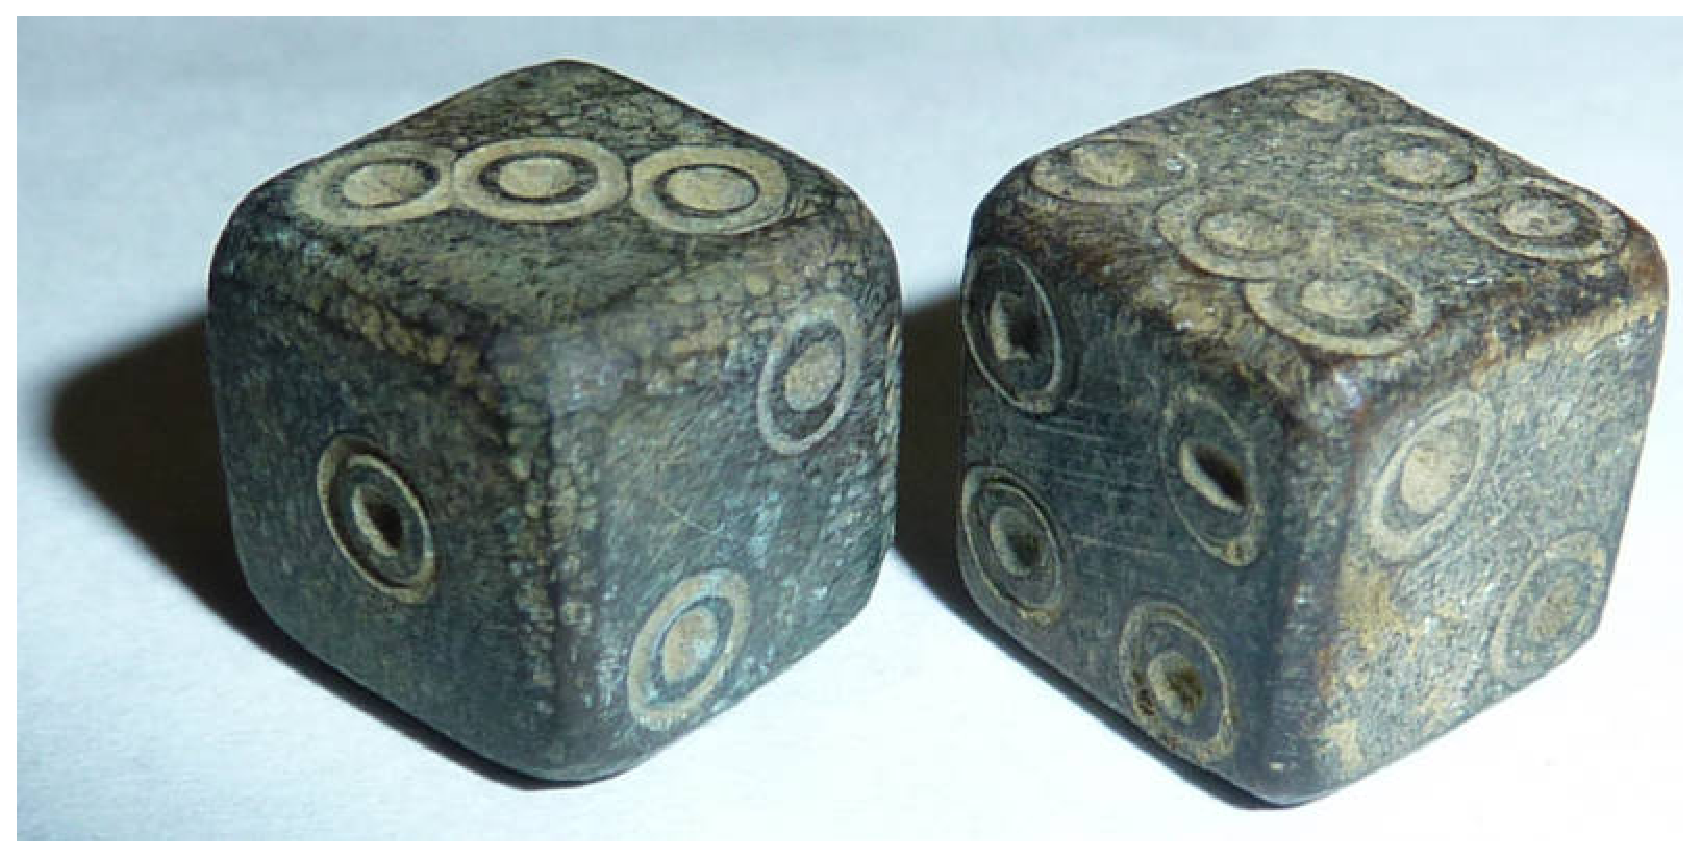
\includegraphics[height=4.2cm]{dice.eps}}
\psframe[linewidth=0.02,linecolor=gray](-6.2,-7)(6.2,2.2)
\psframe[linewidth=0.02,linecolor=gray](-6.15,-6.95)(6.15,2.15)
\rput(0,1.4){\color{myblue}\large Math 207:  Statistics}
\rput(0,0.6){\color{myblue}Chapter 16:  The Law of Averages}
%\psframebox(0,0)(4,4)
\rput(0,-4.5){\scriptsize Dr.~Ralph Wojtowicz}
\rput(0,-5.0){\scriptsize Mathematics Department}
\rput(0,-5.8){
\includegraphics[height=1cm]{su-long.eps}}
%
%\rput(0,-6.5){\scriptsize 17 February 2012}
\end{pspicture}
\end{center}

\end{frame}

%\section[Outline]{}

\addtocounter{page}{-1}
\addtocounter{framenumber}{-1}

{\footnotesize
\frame{\tableofcontents}
}

\section{Law of Averages}
\subsection{Law of Averages}
\begin{frame}[t]\frametitle{Law of Averages}

{\footnotesize

The Law of Averages says that as the size of a random sample increases, the 
difference between the expected percentage of an outcome and the observed percentage
will get smaller (Figure 2).  The difference between the number of occurences of
an outcome and the expected number increases (Figure 1).

\begin{center}
\begin{tabular}{cc}
\scalebox{0.7}{\begin{pspicture}(1.2,0)(11,4)
\psset{yunit=0.05, xunit=2.25}
\psline[linestyle=dotted](1,0)(4,0)
\rput[t](2.5,80){\textbf{Figure 1}}
\rput(2.5,65){$\mbox{EV}_{\mbox{\scriptsize sum}} = n\times\mbox{AV}_{\mbox{\scriptsize box}}$}
\rput(2.56,55){$\mbox{SE}_{\mbox{\scriptsize sum}} = \sqrt{n}\times\mbox{sd}_{\mbox{\scriptsize box}}$}
\psline(1.000000, -1)(1.301030, 0)(1.477121, 2)(1.602060, 1)(1.698970, 0)(1.778151, -1)(1.845098, -3)(1.903090, -5)(1.954243, -5)(2.000000, -6)(2.301030, -2)(2.477121, -4)(2.602060, -1)(2.698970,  5)(2.778151, 12)(2.845098, 18)(2.903090, 13)(2.954243, 8)(3.000000, 2)(3.301030, 13)(3.477121, 10)(3.602060, 29)(3.698970, 33)(3.778151, 9)(3.845098, 16)(3.903090, 34)(3.954243, 38)(4.000000, 67)
\psset{linewidth=0.02}
%
\psline(1,-20)(0.95,-20)\rput[r](0.92,-20){-20}
\psline(1,0)(0.95,0)    \rput[r](0.92,0){0}
\psline(1,20)(0.95,20)  \rput[r](0.92,20){20}
\psline(1,40)(0.95,40)  \rput[r](0.92,40){40}
\psline(1,60)(0.95,60)  \rput[r](0.92,60){60}
\psline(1,80)(0.95,80)  \rput[r](0.92,80){80}
\psline(1,-20)(1,80) % y axis
\rput{90}(0.4,30){Number of Heads Minus}
\rput{90}(0.6,30){Half the Number of Tosses}
%
\psline(1,-20)(1,-24)\rput[t](1,-26){10}
\psline(2,-20)(2,-24)\rput[t](2,-26){100}
\psline(3,-20)(3,-24)\rput[t](3,-26){1,000}
\psline(4,-20)(4,-24)\rput[t](4,-26){10,000}
\psline(1,-20)(4,-20) % x axis
\rput(2.5,-40){Number of Tosses}
\end{pspicture}}
&
\scalebox{0.7}{\begin{pspicture}(3,0)(12,4)
\psset{yunit=0.05, xunit=2.25}
\psline[linestyle=dotted](1,30)(4,30)
\rput[t](2.5,80){\textbf{Figure 2}}
\rput(2.5,65){$\mbox{EV}_{\mbox{\scriptsize av}} = \mbox{AV}_{\mbox{\scriptsize box}}$}
\rput(2.65,55){$\mbox{SE}_{\mbox{\scriptsize av}} = \mbox{sd}_{\mbox{\scriptsize box}}\,/\sqrt{n}$}
\psline(1.000000, -20)(1.301030, 30)(1.477121, 63.3)(1.602060, 42.5)(1.698970, 30)(1.778151, 21.67)(1.845098, 8.57)(1.903090, -1.25)(1.954243, 2.22)(2.000000, 0)(2.301030, 25)(2.477121, 23.3)(2.602060, 28.75)(2.698970,  35)(2.778151, 40)(2.845098, 42.86)(2.903090, 38.125)(2.954243, 34.44)(3.000000, 31)(3.301030, 33.25)(3.477121, 31.67)(3.602060, 33.625)(3.698970, 33.3)(3.778151, 30.75)(3.845098, 31.14)(3.903090, 32.125)(3.954243, 32.111)(4.000000, 33.35)
\psset{linewidth=0.02}
%
\psline(1,-20)(0.95,-20)\rput[r](0.92,-20){-10}
%\psline(1,0)(0.95,0)    \rput[r](0.92,0){0}
\psline(1,5)(0.95,5)  \rput[r](0.92,5){-5}
\psline(1,30)(0.95,30)  \rput[r](0.92,30){0}
\psline(1,55)(0.95,55)  \rput[r](0.92,55){5}
\psline(1,80)(0.95,80)  \rput[r](0.92,80){10}
\psline(1,-20)(1,80) % y axis
%\rput{90}(0.45,30){Number of Heads Minus}
\rput{90}(0.6,30){Percentage of Heads $-$ 50\%}
%
\psline(1,-20)(1,-24)\rput[t](1,-26){10}
\psline(2,-20)(2,-24)\rput[t](2,-26){100}
\psline(3,-20)(3,-24)\rput[t](3,-26){1,000}
\psline(4,-20)(4,-24)\rput[t](4,-26){10,000}
\psline(1,-20)(4,-20) % x axis
\rput(2.5,-40){Number of Tosses}
\end{pspicture}}
\end{tabular}
\end{center}}

\end{frame}

\begin{frame}
\frametitle{Examples}

\footnotesize 
\begin{itemize}
\item<2-> A coin is tossed and you win \$1 if there are more than 70\% heads.  Which is better, 10 tosses or 100?  {\color{blue} 10}.
\item<3-> A coin is tossed and you win \$1 if there are more than 40\% heads.  Which is better, 10 tosses or 100?  {\color{blue} 100}.
\item<4-> A coin is tossed and you win \$1 if there are between 49.999\% and 50.001\% heads.  Which is better, 10 tosses or 100?  {\color{blue} 100}.
\item<5-> A coin is tossed and you win \$1 if there are at most 45\% heads or more than 55\% heads.  Which is better, 10 tosses or 100?  {\color{blue} 10}.
\item<6-> A coin is tossed and you win \$1 if there are exactly 50\% heads.  Which is better, 10 tosses or 100?  {\color{blue} 10}.
\item<7-> A die is rolled and you win \$1 if at least 20\% of the rolls are 5s.  Which is better, 
10 rolls or 100? {\color{blue}10}.
\item<8-> A die is rolled and you win \$1 if between 16\% and 17\% of the rolls are 5s.  Which is better, 
10 rolls or 100? {\color{blue}100}.
\item<9-> A die is rolled and you win \$1 if exactly 1/6 of the rolls are 5s.  Which is better, 
12 rolls or 120? {\color{blue}12}.
\end{itemize}
\end{frame}


\section{Box Models}
\subsection{Box Models}
\begin{frame}{Box Models}

\footnotesize
\begin{itemize}
\item One hundred draws are made at random with replacement from\vspace{-10pt}
\begin{center}
\scalebox{0.7}{\begin{pspicture}(0.2,0.2)(2.5,1.3)
\psframe(0,0)(0.7,0.7)\rput(0.35,0.35){0}
\psframe(1,0)(1.7,0.7)\rput(1.35,0.35){5}
\psframe(2,0)(2.7,0.7)\rput(2.35,0.35){7}
\psline(-0.3,0.9)(-0.3,-0.2)(3,-0.2)(3,0.9)(-0.3,0.9)
\end{pspicture}}
\end{center}
  \begin{itemize}
  \item<2-> \scriptsize  What is the smallest that the sum can be?  {\color{blue}0}\\[3pt]
  \item<3-> \scriptsize What is the largest that the sum can be?  {\color{blue}700}\\[3pt]
  \item<4-> \scriptsize  About what do you expect  the sum to be?\\[2pt]
     {\color{blue}Average of the tickets in
    the box is $\frac{0+5+7}{2}=6$ so 600.}
  \end{itemize}
\item<5-> You plan to roll 100 dice and count the number of 4s.  Make a box model.\vspace{-3pt}
\begin{center}
\scalebox{0.7}{\color{blue}\begin{pspicture}(0.2,0.0)(6.5,1)
\psset{linecolor=blue}
\psframe(0,0)(0.7,0.7)\rput(0.35,0.35){0}
\psframe(1,0)(1.7,0.7)\rput(1.35,0.35){0}
\psframe(2,0)(2.7,0.7)\rput(2.35,0.35){0}
\psframe(3,0)(3.7,0.7)\rput(3.35,0.35){1}
\psframe(4,0)(4.7,0.7)\rput(4.35,0.35){0}
\psframe(5,0)(5.7,0.7)\rput(5.35,0.35){0}
\psline(-0.3,0.9)(-0.3,-0.2)(6,-0.2)(6,0.9)(-0.3,0.9)
\end{pspicture}}\vspace{2pt}
\end{center}
\item<6-> You plan to roll 100,000 dice and count the number of even numbers.  
Make a box model.\vspace{-10pt}
\begin{center}
\scalebox{0.7}{\color{blue}\begin{pspicture}(0.2,0.2)(6.5,1)
\psset{linecolor=blue}
\psframe(0,0)(0.7,0.7)\rput(0.35,0.35){0}
\psframe(1,0)(1.7,0.7)\rput(1.35,0.35){1}
\psframe(2,0)(2.7,0.7)\rput(2.35,0.35){0}
\psframe(3,0)(3.7,0.7)\rput(3.35,0.35){1}
\psframe(4,0)(4.7,0.7)\rput(4.35,0.35){0}
\psframe(5,0)(5.7,0.7)\rput(5.35,0.35){1}
\psline(-0.3,0.9)(-0.3,-0.2)(6,-0.2)(6,0.9)(-0.3,0.9)
\end{pspicture}}
\end{center}
\end{itemize}
\label{lastpage}
\end{frame}

\end{document}


\label{lastpage}
\end{frame}
\end{document}
